
\chapter{Конструкторская часть}\label{Konstruct}
%\addcontentsline{toc}{chapter}{2 Конструкторская часть}

В данном разделе представлены схемы алгоритмов. Так же будут описаны пользовательские структуры данных, 
приведены классы эквивалентности для тестирования реализуемого ПО.

\section{Схемы алгоритмов}\label{SchemaAlg}


\subsection{Схема алгоритма полного перебора}\label{SchemaPoslMatrixMultiply}

На рисунке \ref{ris:schemaposav} показана схема алгоритма полного перебора.

\begin{figure}[H]
  \center{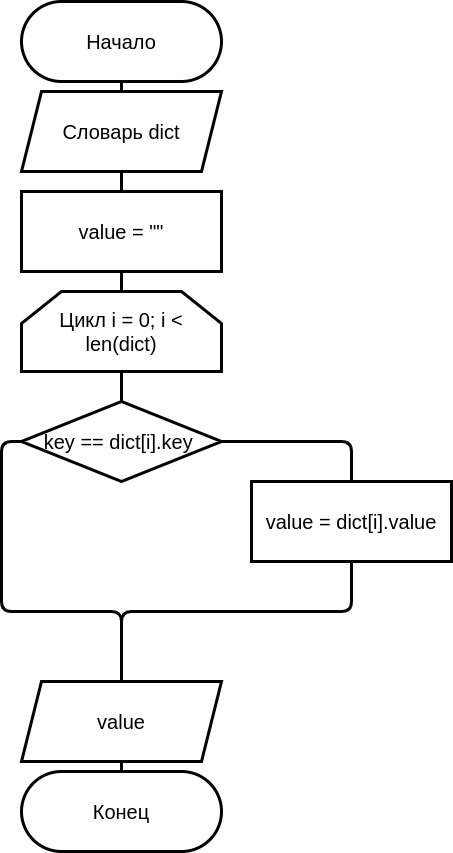
\includegraphics[scale=0.40]{l1.all}}
  \caption{Схема алгоритма полного перебора}
  \label{ris:schemaposav}
\end{figure}

\subsection{Схема алгоритма бинарного поиска}\label{SchemaParRowMatrixMultiply}

На рисунке \ref{ris:schemaparrowav} показана схема алгоритма бинарного поиска.

\begin{figure}[H]
  \center{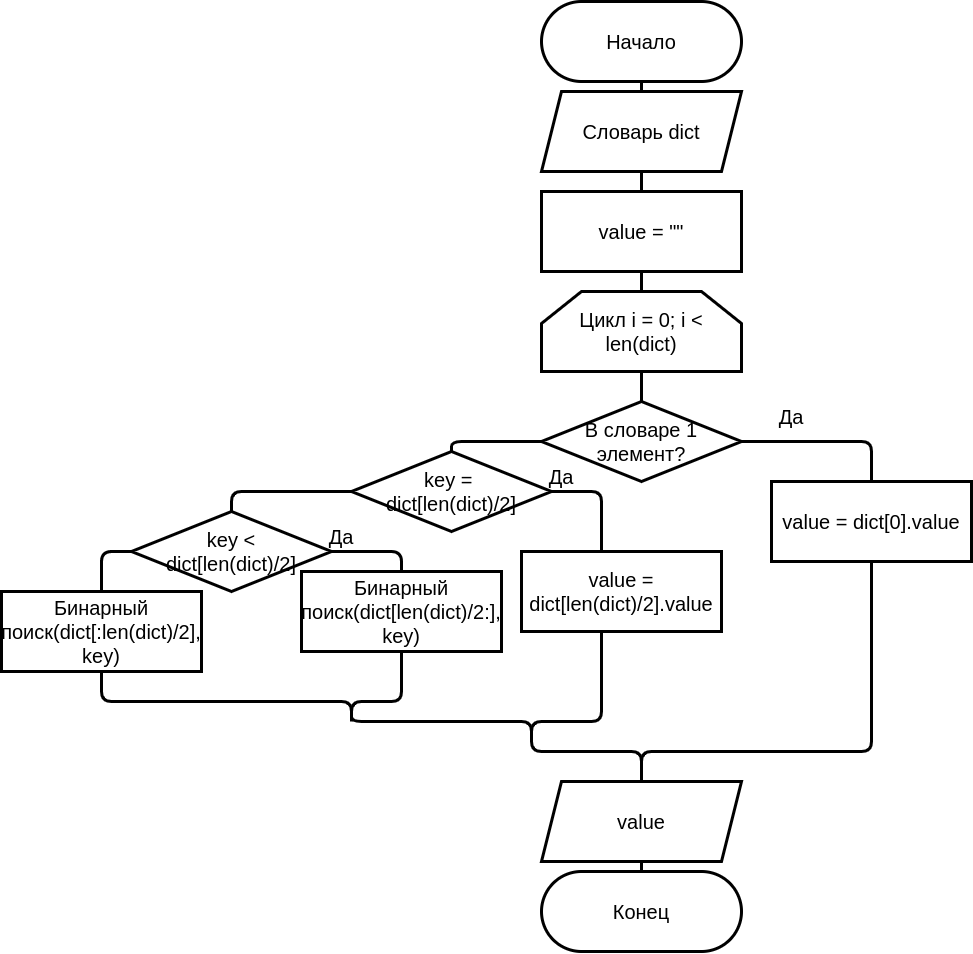
\includegraphics[scale=0.40]{l1.bin}}
  \caption{Схема алгоритма бинарного поиска}
  \label{ris:schemaparrowav}
\end{figure}

\subsection{Схема алгоритма частотного анализа}\label{SchemaParColumnMatrixMultiply}

На рисунке \ref{ris:schemaparcolumnav} показана схема алгоритма частотного анализа.

\begin{figure}[H]
  \center{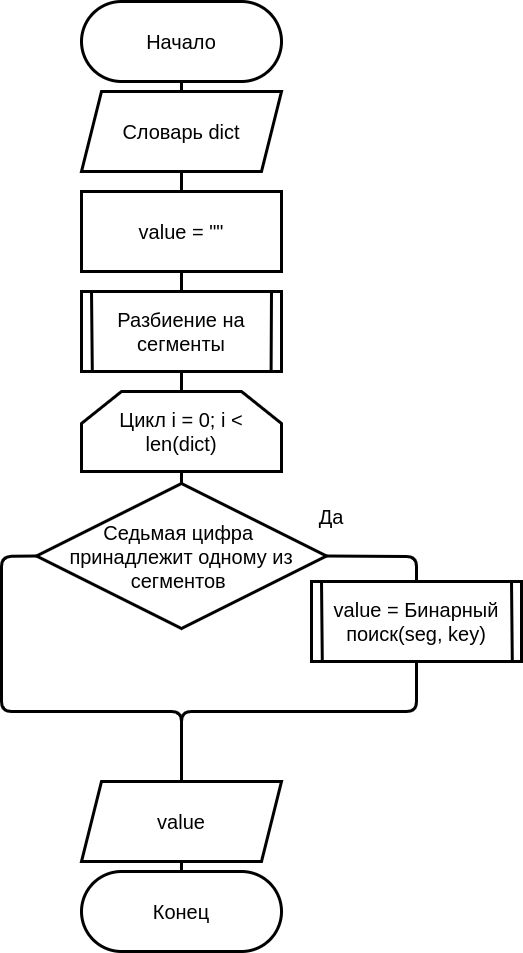
\includegraphics[scale=0.40]{l1.seg}}
  \caption{Схема алгоритма частотного анализа}
  \label{ris:schemaparcolumnav}
\end{figure}


\section{Структуры данных}\label{Structs}

При реализации приведенных алгоритмов потребуется тип данных: словарь. Словарь содержит два поля:

\begin{enumerate}
  \item ключ 
  \item значение
\end{enumerate}

\section{Тестирование}\label{Testing}


Для алгоритмов поиска по словарю можно выделить следующие классы эквивалентности:

\begin{enumerate}
    \item ключа нет в словаре;
    \item первый ключ;
    \item последний ключ;
    \item случайный ключ:
\end{enumerate}

%\subsection{Способы тестирования}\label{TestingMethods}

%При разработке программы удобно использовать следующие методы тестирования:

%\begin{enumerate}
%    \item Модульные тесты 
%    \item Функциональные тесты 
%\end{enumerate}

\section{Вывод конструкторской части}\label{KonstructResult}
На основе данных, полученных в аналитическом разделе, были построены схемы используемых алгоритмов,
выделены необходимые для реализации структуры данных и методы тестирования.

